\documentclass[a4paper, 12pt]{article}
\usepackage[utf8]{inputenc}
\usepackage[T1]{fontenc}
\usepackage[french]{babel}
\usepackage{lmodern}
\usepackage{graphicx, float, svg} 
\usepackage{amsmath, amssymb, amsthm}
\usepackage{listings}
\usepackage[listings,skins]{tcolorbox}
\usepackage{xcolor}

\usepackage[hyphens]{url}
\usepackage[pdfauthor = {{Prénom Nom}}, pdftitle = {{Titredocument}},pdfstartview = Fit, pdfpagelayout =
SinglePage, pdfnewwindow = true, bookmarksnumbered =
true, breaklinks, colorlinks, linkcolor = red, urlcolor =
black, citecolor = cyan, linktoc = all]{hyperref}

\usepackage[a4paper,margin=2.5cm]{geometry}

% \renewcommand{\familydefault}{\sfdefault}
\definecolor{codegreen}{rgb}{0,0.6,0}
\definecolor{codegray}{rgb}{0.5,0.5,0.5}
\definecolor{codepurple}{rgb}{0.58,0,0.82}
\definecolor{codeblue}{rgb}{0.0, 0.4, 0.8}
\definecolor{darkWhite}{rgb}{0.90,0.90,0.90}

\lstdefinestyle{bigCode}{
    backgroundcolor=\color{darkWhite},   
    commentstyle=\color{codegreen},
    keywordstyle=\color{codeblue},
    numberstyle=\tiny\color{codegray},
    stringstyle=\color{codepurple},
    basicstyle=\ttfamily\footnotesize,
    breakatwhitespace=false,         
    breaklines=true,                 
    captionpos=b,                    
    keepspaces=true,                 
    showspaces=false,                
    showstringspaces=false,
    showtabs=false,                  
    tabsize=2,
    language=c,
    morekeywords={free,malloc,nullptr,calloc,memcpy,realloc,bool,size_t,true,false}
}

\hypersetup{
  colorlinks=true,       % Enables colored links
  linkcolor=gray,        % Color for internal links (e.g., \ref and \autoref)
  citecolor=gray,        % Color for citations
  filecolor=gray,        % Color for file links
  urlcolor=gray          % Color for external URLs
}


\lstset{style=bigCode}

\NewTotalTCBox{\commandbox}{ s v }
{verbatim,colupper=black,colback=darkWhite!75!white,colframe=white,left=0pt,boxsep=0px,right=0pt,top=2px,bottom=2px}
{\IfBooleanT{#1}{\textcolor{red}{\ttfamily\bfseries > }}%
\lstinline[language=c,morekeywords={free,malloc,nullptr,calloc,memcpy,realloc,bool,size_t,true,false},keywordstyle=\color{codeblue}\bfseries]^#2^}

\newcommand{\code}{\commandbox}

\title{Distance de Jaccard}
\author{Maysaloon BILAL \& Tristan GROULT}
\date{\today}

\begin{document}

\begin{figure}[t]
    \centering
    \begin{minipage}{0.3\textwidth}
        \centering
        
\includegraphics[width=1\textwidth]{logo_univ.png}
    \end{minipage}
    \hfill
    \begin{minipage}{0.3\textwidth}
        \centering
        
\includegraphics[width=1\textwidth]{ufr_logo.png}
    \end{minipage}
\end{figure}

\maketitle

\clearpage\setcounter{page}{2}

{
\hypersetup{hidelinks} % Sommaire en "noir"
\renewcommand{\contentsname}{Sommaire}
\tableofcontents % Affichage du sommaire
}

\clearpage

\section{Introduction}


Ce projet consiste à développer un programme en langage C permettant de calculer la distance de Jaccard entre plusieurs fichiers texte, afin d'analyser leur similarité lexicale. La distance de Jaccard est une valeur comprise entre 0 et 1 : plus elle est proche de 0, plus les fichiers sont différents, et plus elle est proche de 1, plus ils sont similaires.

La distance de Jaccard entre deux ensembles $A$ et $B$ est définie par la formule :
$$
\text{Distance de Jaccard}(A, B) = 1 - \frac{|A \cap B|}{|A \cup B|}
$$

Le programme propose plusieurs modes d'affichage ainsi que des calculs personnalisés.  
Il est possible de mesurer la similarité entre les fichiers à l'aide de l'indice de Jaccard, que nous désignerons par la suite par \textit{Calcul de Jaccard}.  
Il est également possible d'afficher un graphe représentant l'appartenance des mots à leur(s) fichier(s), que nous nommerons \textit{Graphe de Jaccard}.  
Nous utiliserons le terme \textit{Calcul de Jaccard} pour faire référence à la réalisation ou la préparation de ces deux opérations.

Pour gérer efficacement les mots extraits des fichiers, nous avons utilisé une table de hachage. Sa gestion — ajout, suppression, affichage du graphe, etc. — est implémentée dans le module \code{jaccard}. Ce projet s'appuie également sur deux autres modules : le module \code{word} \autoref{word}, dédié à la création et la manipulation des mots, et le module \code{opt} \autoref{opt}, responsable du traitement des options en ligne de commande.

L'ensemble de ces composants est intégré et testé dans le fichier principal \code{main.c}, qui constitue le point d'entrée du programme.


\section{Conception et implémentation}

Dans cette section, nous expliquons les différentes étapes et approches utilisées pour implémenter le programme. Nous détaillerons la conception des modules, la gestion des fichiers et l'utilisation de la table de hachage.

\subsection{Module word}

\label{word}

Le module \code{word} a pour objectif de construire dynamiquement un mot caractère par caractère, afin de faciliter son traitement sans avoir à connaître sa taille à l'avance. Ce module est utilisé lors de la lecture des fichiers afin d'extraire chaque mot individuellement.

\subsubsection{Spécification}

Pour cela, nous utilisons une structure de données définie dans la \autoref{fig:word_schema}. Cette structure permet de stocker un mot, d'en gérer dynamiquement la taille, et de le manipuler facilement sans risque de dépassement mémoire. 

\begin{figure}[H]
\centering
\begin{tcolorbox}[enhanced,
colback=white,
colframe=codeblue,
fonttitle=\bfseries,
title=Schéma,
boxrule=2pt,
width=0.8\textwidth]
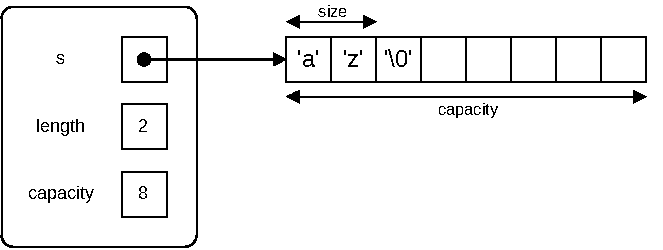
\includegraphics[width=\textwidth]{word_schema.pdf}
\end{tcolorbox}
\caption{Schéma de la structure word}
\label{fig:word_schema}
\end{figure}

\subsubsection{Implantation}

Lors de l'implémentation, nous avons défini une structure \code{struct word} (\autoref{fig:structure_word}) pour représenter dynamiquement un mot. Elle est composée de trois champs :

\begin{itemize}
\item Un champ \code{s} de type \code{char *} qui pointe vers un tableau de caractères contenant le mot.
\item Un champ \code{length} de type \code{size_t} qui représente la longueur actuelle du mot.
\item Un champ \code{capacity} de type \code{size_t} qui correspond à la taille totale allouée pour le mot.
\end{itemize}

Nous avons choisi une approche avec allocation mémoire dynamique, ce qui permet de s'adapter à la longueur des mots rencontrés, en multipliant par la constante \code{CAPACITY_MUL} la capacité du mot lorsque celle-ci est atteinte.

\begin{figure}[h]
\centering
\begin{tcolorbox}[center upper,
enhanced,
colback=darkWhite,
boxrule=0pt,
frame hidden,
width=0.4\textwidth]
\begin{lstlisting}[style=bigCode]
struct word {
    char *s;
    size_t length;
    size_t capacity;
};
\end{lstlisting}
\end{tcolorbox}
\caption{Structure word}
\label{fig:structure_word}
\end{figure}

Nous avons développé plusieurs fonctions pour interagir avec ce module :

\begin{itemize}
\item \code{word_init()} : Initialise un mot vide en allouant une capacité minimale définie par la constante \code{CAPACITY_MIN}, et met la longueur à zéro.

\item \code{word_add()} : Ajoute un caractère à la fin du mot. Si la capacité est atteinte, elle est doublée avec \code{realloc()} pour permettre l'ajout de nouveaux caractères.

\item \code{word_reinit()} : Réinitialise le mot en mettant sa longueur à zéro, ce qui permet de le réutiliser sans réallouer de mémoire.

\item \code{word_get()} : Renvoie un pointeur vers la chaîne de caractères actuelle.

\item \code{word_get_clean()} : Copie le contenu réel du mot dans une destination passée en paramètre, sans les éventuels caractères résiduels.

\end{itemize}



\subsection{Module opt}
\label{opt}

Le module \code{opt} a pour objectif de gérer les options de la ligne de commande, en les analysant puis en les restituant sous une forme exploitable par le reste du programme.
Dans le cadre de ce projet, les options suivantes sont nécessaires :

\begin{itemize}
\item \code{-g} : Affiche le graphe de Jaccard.
\item \code{-p} : Ignore les caractères de ponctuation lors de l'analyse.
\item \code{-iVALUE} : Spécifie la longueur maximale des mots.
\item \code{-} : Utilise l'entrée standard comme source.
\item \code{--} : Indique que l'argument suivant est un nom de fichier.
\item \code{-u} : Affiche les informations d'utilisation de l'exécutable.
\item \code{-v} : Affiche la version de l'exécutable.
\item \code{-?} : Affiche l'aide de l'exécutable.
\end{itemize}

\subsubsection{Spécification}

Pour représenter les options analysées, nous utilisons une structure de données illustrée dans la \autoref{fig:opt_schema}.
Nous avons choisi de limiter le nombre de fichiers grâce à une constante nommée \code{MAX_FILES}. Ce choix permet d'assurer une consommation mémoire bornée et facilite l'intégration avec les contraintes d'implémentation du module \code{jaccard}.

\begin{figure}[H]
\centering
\begin{tcolorbox}[enhanced,
colback=white,
colframe=codeblue,
fonttitle=\bfseries,
title=Schéma,
boxrule=2pt,
width=0.8\textwidth]
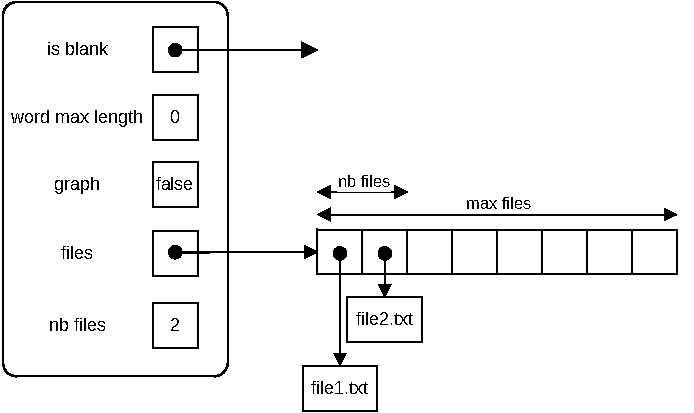
\includegraphics[width=\textwidth]{opt_schema.pdf}
\end{tcolorbox}
\caption{Schéma de la structure opt}
\label{fig:opt_schema}
\end{figure}

\subsubsection{Implémentation}

L'implémentation repose sur l'utilisation d'une structure \code{struct opt}, définie comme suit (\autoref{fig:structure_opt}) :

\begin{itemize}
\item \code{isBlank} : Pointeur vers une fonction \code{int(int)} déterminant les caractères séparateurs de mots.
\item \code{word_max_length} : Entier définissant la longueur maximale d'un mot (0 signifie aucune limite ; valeur par défaut : 0).
\item \code{graph} : Booléen indiquant si le graphe de Jaccard doit être affiché.
\item \code{files} : Tableau de chaînes de caractères représentant les noms des fichiers à analyser.
\item \code{nb_files} : Nombre de fichiers fournis en argument.
\end{itemize}

\begin{figure}[h]
\centering
\begin{tcolorbox}[center upper,
enhanced,
colback=darkWhite,
boxrule=0pt,
frame hidden,
width=0.5\textwidth]
\begin{lstlisting}[style=bigCode]
struct opt {
    int (*isBlank)(int);
    int word_max_length;
    bool graph;
    char const **files;
    int nb_files;
};
\end{lstlisting}
\end{tcolorbox}
\caption{Structure opt}
\label{fig:structure_opt}
\end{figure}

Afin de permettre une gestion homogène de l'entrée standard, nous la représentons sous la forme d'une chaîne vide (\code{""}), en la définissant via une macro \code{STDIN}. Cette chaîne est utilisée comme nom de fichier, en tirant parti du fait qu'aucun système courant ne l'autorise comme nom valide.

Seules les options courtes ont été implémentées, comme listé plus haut. Pour l'option \code{-iVALUE}, la valeur doit être directement collée à l'option (par exemple \code{-i3}), l'espacement (\code{-i 3}) n'étant pas pris en charge.

Enfin, toutes les options sont définies via des macros constantes. Le préfixe des options courtes est également paramétrable, ce qui rend l'ensemble du module facilement adaptable à d'autres conventions si nécessaire.


\subsection{Module Jaccard}

Le module \code{jaccard} a pour objectif de réaliser le calcul de Jaccard en donnant la possibilité d'ajouter des mots au calcul ainsi que de gérer l'affichage du graphe ou le calcul de la distance.

\subsubsection{Spécification}

Pour réaliser cela, nous utilisons une structure de données définie dans la \autoref{fig:jaccard_shema}. Cette structure permet de sauvegarder les éléments utilisés pour réaliser le calcul de la distance ainsi que les autres structures que nous avons décidé d'utiliser. 

\begin{figure}[H]
\centering
\begin{tcolorbox}[enhanced,
colback=white,
colframe=codeblue,
fonttitle=\bfseries,
title=Schéma,
boxrule=2pt,
width=0.8\textwidth]
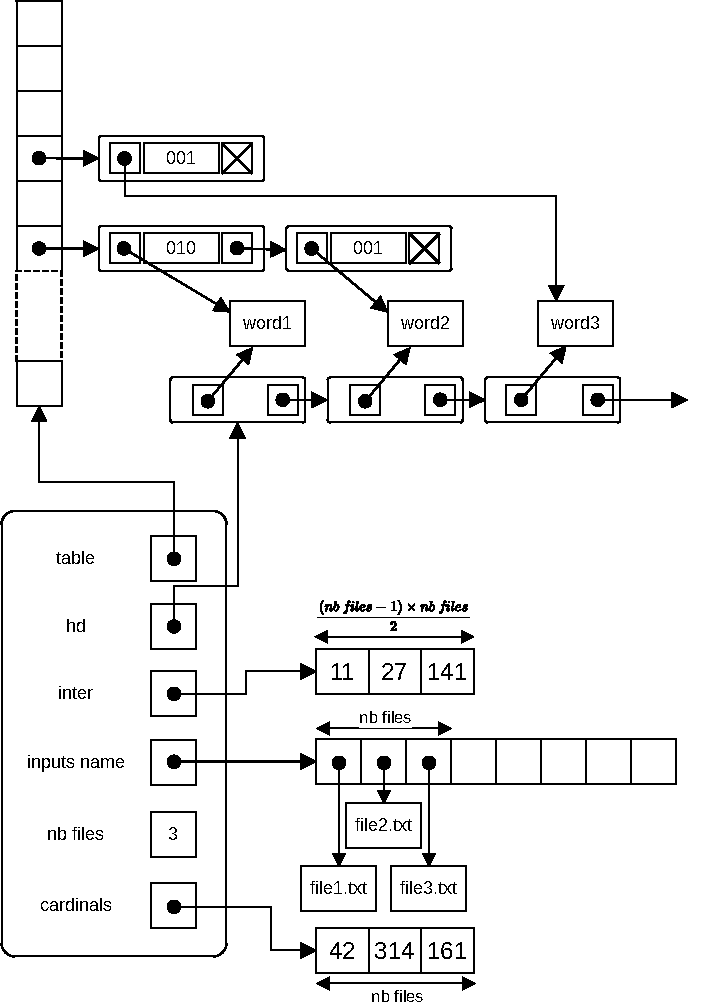
\includegraphics[width=\textwidth]{jaccard_schema.pdf}
\end{tcolorbox}
\caption{Schéma de la structure jaccard}
\label{fig:jaccard_shema}
\end{figure}

Pour réaliser le calcul de Jaccard, nous avons besoin : 

\begin{itemize}
    \item D'un champ $nb\ files$ permettant de connaître le nombre de fichiers utilisés pour le calcul de Jaccard courant.
    \item D'un tableau $inputs\ name$ contenant le nom des fichiers utilisés lors de l'affichage du graphe de Jaccard ou du calcul de Jaccard. L'ordre des fichiers est important car plusieurs autres endroits utilisent ce même ordre pour représenter ces mêmes fichiers. On considère que ce tableau de noms de fichiers est de taille $nb\ files$.
    \item D'un tableau constitué des cardinaux de la forme ensembliste de chaque fichier. Le cardinal à l'indice $i$ est celui du fichier d'indice $i$ dans inputs name. Ce tableau est donc de taille $nb \ files$.
    
    \item D'un tableau pour stocker les cardinaux des intersections entre chaque paire de fichiers. Chaque case du tableau représente une paire de fichiers différents. La taille totale du tableau est égale au nombre de paires possibles, soit $\frac{n \cdot (n - 1)}{2}$ si on a $n$ fichiers.
    
    Pour deux fichiers avec les indices $i$ et $j$ (avec $i < j$), l'indice $idx$ de la case du tableau correspondant au cardinal de leur intersection est :  
    $$
        idx(i, j) = i \cdot nb\ files - \frac{i \cdot (i + 1)}{2} + (j - i - 1)
    $$
    Cette formule transforme un couple d'indices de fichiers $(i, j)$ en un indice unique dans le tableau, ce qui permet de toujours savoir à quelle intersection correspond chaque case.

    \item Un champ $table$ contenant une table de hachage dans laquelle les mots vont pouvoir être recherchés et ajoutés durant le calcul de Jaccard.
    
    \item Le champ $hd$ contenant une liste dynamique en mesure d'accueillir tous les mots qui sont ajoutés au calcul de Jaccard. C'est sur cette liste dynamique que doit être réalisé le tri si nécessaire car une table de hachage n'est pas triée.
\end{itemize}

La mise à jour du tableau des cardinaux des intersections est réalisée à chaque ajout d'un nouveau mot au calcul de Jaccard en suivant l'algorithme suivant : 

\begin{figure}[h]
\centering
\begin{tcolorbox}[center upper,
enhanced,
colback=darkWhite,
boxrule=0pt,
frame hidden,
width=0.8\textwidth]
\begin{lstlisting}[style=bigCode,language=]
Soit M le mot
Soit T le bitmap du mot M
Soit F le fichier dans lequel on a lu M
Soit j l'indice de F
Soit I le tableau des cardinaux des intersections
Soit i = 0

tant que i < j faire
    si M[i] = 1 alors
         I[idx(i, j)] <- I[idx(i, j)] + 1
    fin si
    i <- i + 1
fin tant que
\end{lstlisting}
\end{tcolorbox}
\caption{Algorithme de mise à jour du tableau des cardinaux des intersections }
\label{fig:algo_inter}
\end{figure}

Voici un exemple de l'application de l'algorithme.

\begin{figure}[H]
\centering
\begin{tcolorbox}[enhanced,
colback=white,
colframe=codeblue,
fonttitle=\bfseries,
title=Exemple,
boxrule=2pt,
width=0.8\textwidth]
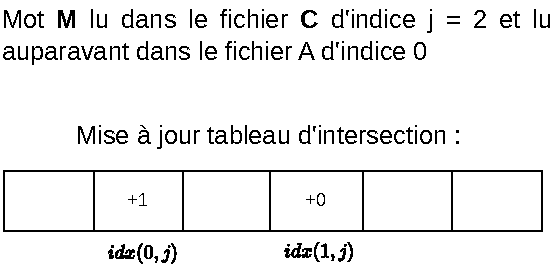
\includegraphics[width=\textwidth]{algo_inter.pdf}
\end{tcolorbox}
\caption{Exemple mise à jour du tableau des cardinaux des intersections}
\label{fig:algo_inter}
\end{figure}


\subsubsection{Implémentation}

Pour la réalisation de ce module nous avons développé de nombreuses fonctions afin de créer un calcul de Jaccard, d'ajouter des mots au calcul et finalement de procéder à l'affichage du calcul de Jaccard et du graphe de Jaccard.

\begin{figure}[h]
\centering
\begin{tcolorbox}[center upper,
enhanced,
colback=darkWhite,
boxrule=0pt,
frame hidden,
width=0.5\textwidth]
\begin{lstlisting}[style=bigCode]
struct jcrd {
    hashtable *table;
    holdall *hd;
    const char **inputs_name;
    size_t *inter;
    bool graph;
    int nb_files;
    size_t *cardinals;
};
\end{lstlisting}
\end{tcolorbox}
\caption{Exemple d'utilisation des masques sur une bitmap}
\label{fig:exemple_bits}
\end{figure}

Nous avons rencontré un problème sur le calcul de l'appartenance de chaque mot à son/ses fichiers. Nous avons décidé d'utiliser une bitmap afin de représenter ce tableau d'appartenance. La table de hachage a comme champ \code{ref} un pointeur de type \code{const void *}. Pour limiter notre nombre d'allocations, nous avons décidé d'écrire directement notre bitmap sur l'adresse du pointeur plutôt que d'allouer un nombre servant de bitmap. Pour réaliser cette manipulation, nous utilisons le type \code{uint64_t} permettant un codage assuré sur 64 bits, la taille d'une adresse mémoire. L'utilisation de ce type est aussi intéressante pour pouvoir caster ce nombre en une adresse grâce aux forceurs de type \code{(void *) (uintptr_t)} qui est compatible avec le type \code{const void *}. Nous vérifions la présence d'un bit à 0 à un indice grâce à des masques. Voici par exemple un masque permettant de détecter si le bit d'indice $i$ est à 0 et permettant de mettre le bit d'indice $i$ à 1 comme vous pouvez le voir dans l'exemple suivant : \autoref{fig:exemple_bits}


\begin{figure}[h]
\centering
\begin{tcolorbox}[center upper,
enhanced,
colback=darkWhite,
boxrule=0pt,
frame hidden,
width=1\textwidth]
\begin{lstlisting}[style=bigCode]
bitmap & (1ULL << i) // Detecte si le bit d indice i est a 1
bitmap |= (1ULL << i) // Met a 1 le bit d indice i
\end{lstlisting}
\end{tcolorbox}
\caption{Exemple d'utilisation des masques sur une bitmap}
\label{fig:exemple_bits}
\end{figure}

% Voici un exemple de cas pour la détection et mise à jour de la bitmap


\begin{itemize}
    \item \code{jaccard_init()} Initialise un nouveau calcul de Jaccard pour le nombre de fichiers et noms passés en paramètre.
    \item \code{jaccard_add()} traite un mot lu dans un fichier, et met à jour à la fois la table de hachage, les cardinaux des fichiers, et le tableau des cardinaux des intersections. Voir \autoref{fig:intersection} pour un exemple.
    \item \code{jcrd_print_distance()} Calcule et affiche les distances de Jaccard entre toutes les paires de fichiers analysés.
    Pour chaque paire de fichiers $(i, j)$ avec (avec $i < j$), la fonction effectue les opérations suivantes :

    \begin{itemize}
        \item calcul de l'union pour les fichiers d'indices $i$ et $j$
        $$
        CardUnion(i,j) = cardinals[i] + cardinals[j] - inter[idx(i,j)]
        $$
        \item Calcul de la distance de Jaccard par application de la formule :
        $$
        distance(i,j) = 1 - \frac{inter[idx(i,j)]}{CardUnion(i,j)}
        $$

    \end{itemize}
    \item \code{jcrd_print_graph()} Affiche sur la sortie standard le graphe de Jaccard. Pour cela, les mots ont été préalablement triés grâce à la fonction de comparaison \code{strcol} passée en paramètre de la fonction \code{holdall_sort}
\end{itemize}

\begin{figure}[H]
\centering
\begin{tcolorbox}[enhanced,
colback=white,
colframe=codeblue,
fonttitle=\bfseries,
title=Exemple,
boxrule=2pt,
width=0.8\textwidth]
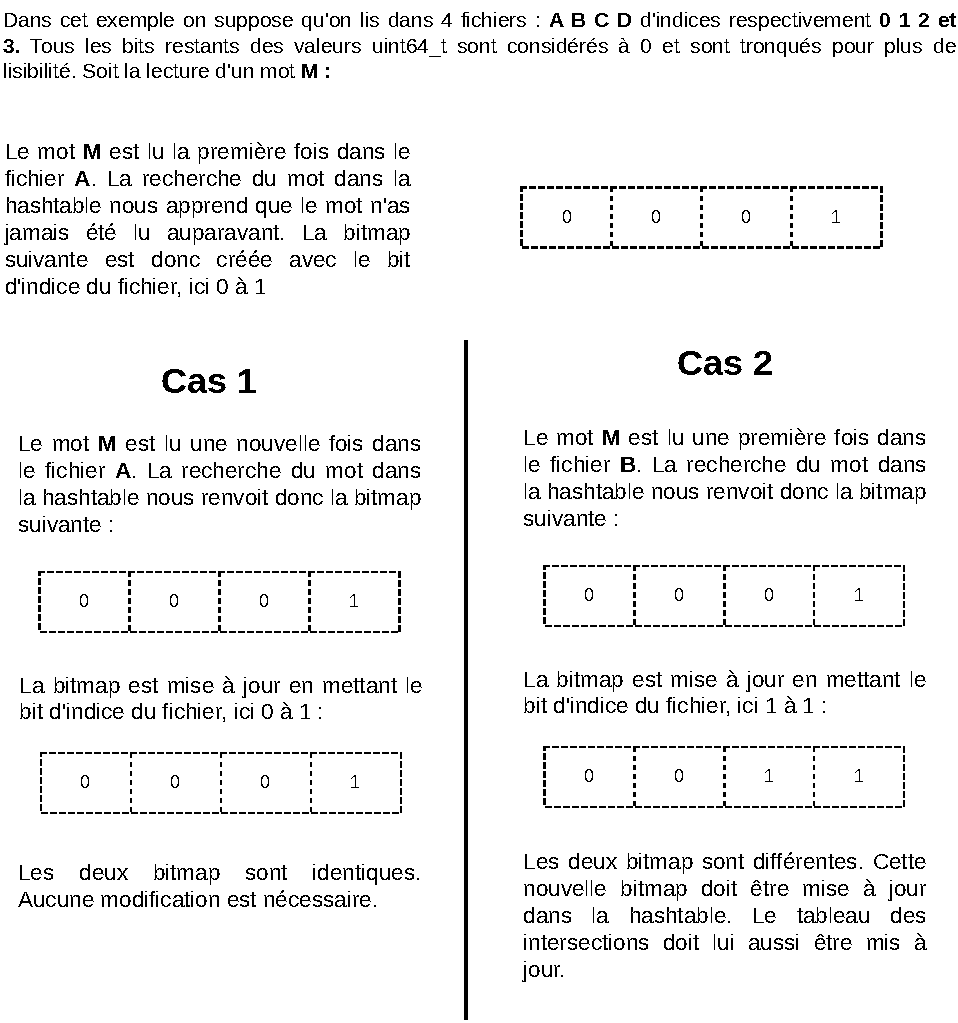
\includegraphics[width=\textwidth]{intersections.pdf}
\end{tcolorbox}
\caption{Schéma du tableau d'intersections}
\label{fig:intersection}
\end{figure}

\subsection{Module holdall}

L'implantation de ce module n'a pas été modifiée à l'exception de l'extension qui a été implémentée et qui comprend la fonction de tri \code{holdall_sort} permettant de trier le trousseau. Nous avons choisi d'implémenter pour ce tri, l'algorithme de tri fusion afin d'assurer une complexité en tout cas de $O(n \log n)$.

\subsection{Main}
\subsubsection {Implémentation}

\begin{itemize}
  \item Le programme commence par initialiser les modules \code{opt}, \code{jaccard}, \code{word} et \code{holdall}.

  \item Chaque mot des fichiers est lu et ajouté au calcul de Jaccard

  \item Une fois la lecture de chaque fichier terminée, celui-ci est fermé (ou réinitialisé dans le cas de \texttt{stdin} avec \code{rewind(stdin)}).

  \item À la fin de la lecture, si l'option d'affichage de graphe n'est pas activée, le programme affiche les distances de Jaccard calculées entre toutes les paires de fichiers. Sinon, il affiche le graphe de Jaccard.

  \item Enfin, toutes les structures utilisées sont libérées proprement (\code{word}, \code{jaccard} et \code{opt} et \code{holdall}) pour éviter les fuites mémoire et on renvoie \code{EXIT_SUCCESS}. Et toute éventuelle erreur au cours de l'exécution arrête le programme en affichant le type de l'erreur et en libérant toutes les ressources allouées jusque-là. Dans ce cas la fonction renvoie \code{EXIT_FAILURE}.
\end{itemize}

\section{Améliorations possibles}

L'utilisation de \code{uint64_t} avec le codage de l'appartenance des mots à leur fichier directement sur l'adresse fonctionne uniquement pour les systèmes en 64 bits. Une amélioration possible serait de gérer lors de la compilation, grâce à la définition d'une macro constante, le nombre de fichiers maximum pris en compte et d'adapter en conséquence le codage de l'appartenance des mots à leur fichier afin de s'adapter aux différents codages des adresses des machines.

\end{document}